\subsection*{4 a)}
\textbf{Bruk funksjonen streamfun i et skript,\sout{strlin.m eller} strlin.py,
 som plotter konturlinjer for $\psi$ når $n = 5 \land n =30$.}
 \footnote{$\land$ er kul, men feil å bruke i denne sammenhengen.}

\begin{figure}[H]
    \centering
    \begin{subfigure}{0.3\textwidth}
        \centering
        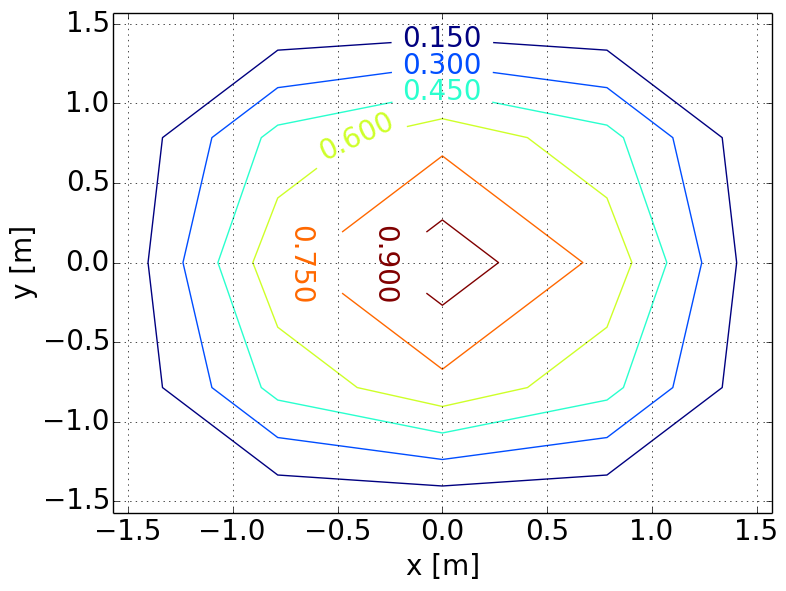
\includegraphics[width=\linewidth]{../4a_0_0,5_5.png}
        \caption{}
    \end{subfigure}%
    ~
    \begin{subfigure}{0.3\textwidth}
        \centering
        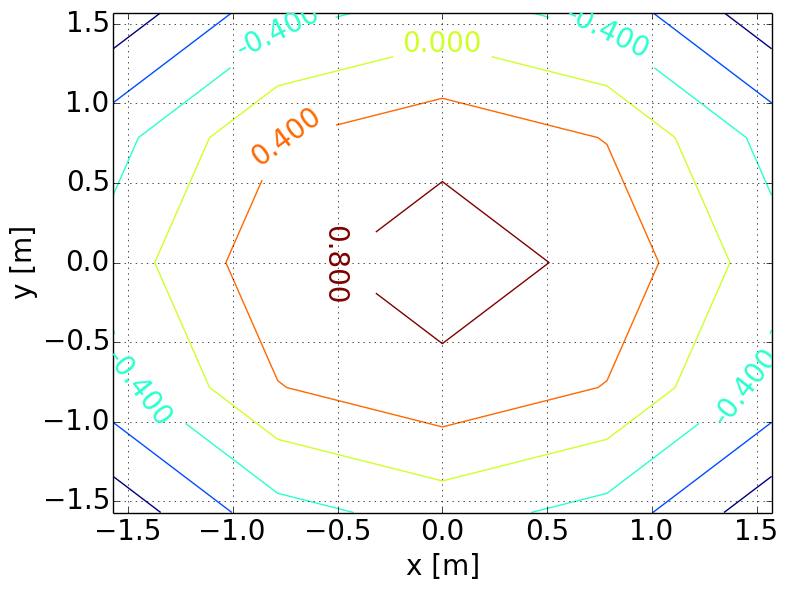
\includegraphics[width=\linewidth]{../4a_1_0,5_5.png}
        \caption{}
    \end{subfigure}
    ~
    \begin{subfigure}{0.3\textwidth}
        \centering
        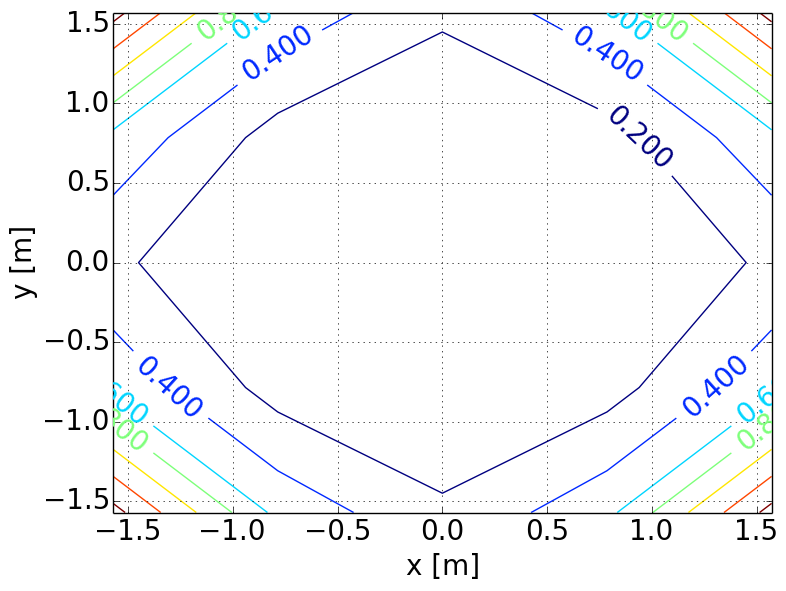
\includegraphics[width=\linewidth]{../4a_2_0,5_5.png}
        \caption{}
    \end{subfigure}
    \caption{Figurene viser $|x| < \frac{\pi}{2}$ og
    $|y| < \frac{\pi}{2}$ med $n = 5$.
    \color{blue} a) \color{black}
     viser konturlinjene
    til $\psi$.
    \color{blue} b) \color{black}
     viser konturlinjene til Taylor approksimasjon
    fra 3 e).
    \color{blue} c) \color{black}
     viser konturlinjene til forskjellen mellom a) og b). }
    \label{fig_4a_first}
\end{figure}

\begin{figure}[H]
    \centering
    \begin{subfigure}{0.3\textwidth}
        \centering
        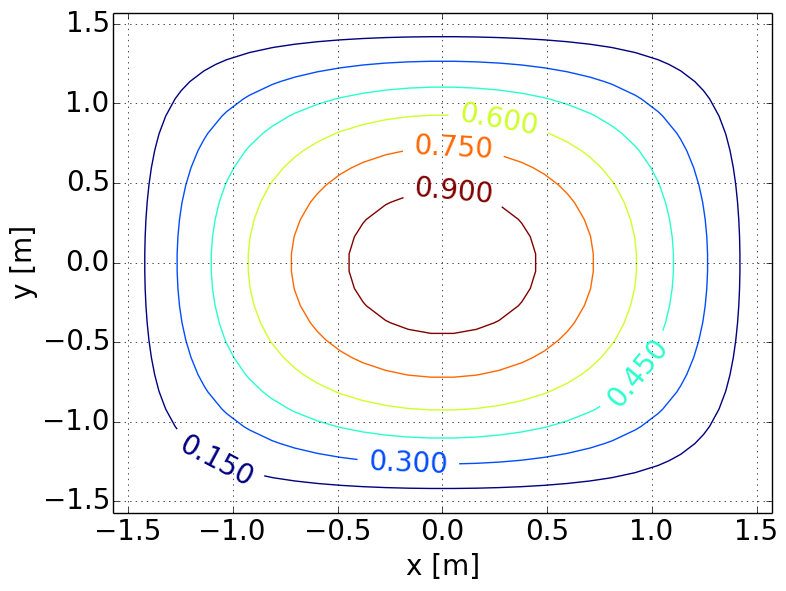
\includegraphics[width=\linewidth]{../4a_0_0,5_30.png}
        \caption{}
    \end{subfigure}%
    ~
    \begin{subfigure}{0.3\textwidth}
        \centering
        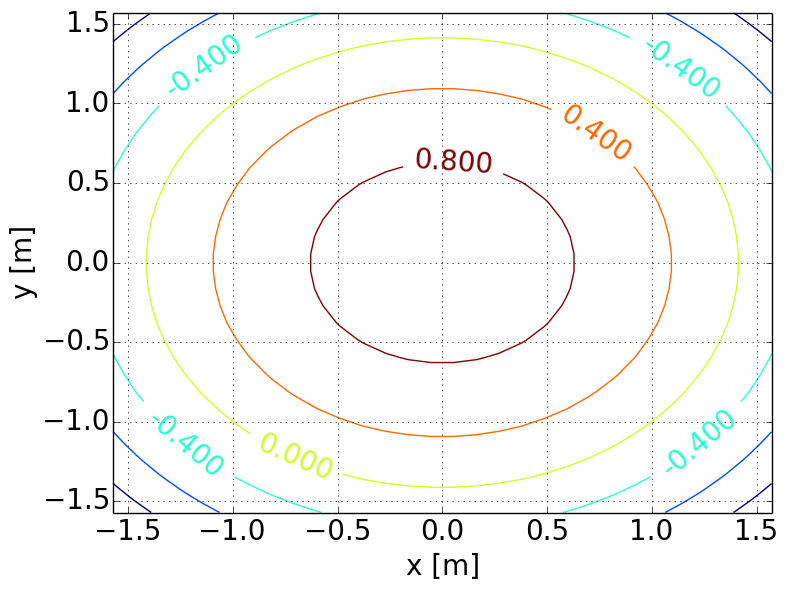
\includegraphics[width=\linewidth]{../4a_1_0,5_30.png}
        \caption{}
    \end{subfigure}
    ~
    \begin{subfigure}{0.3\textwidth}
        \centering
        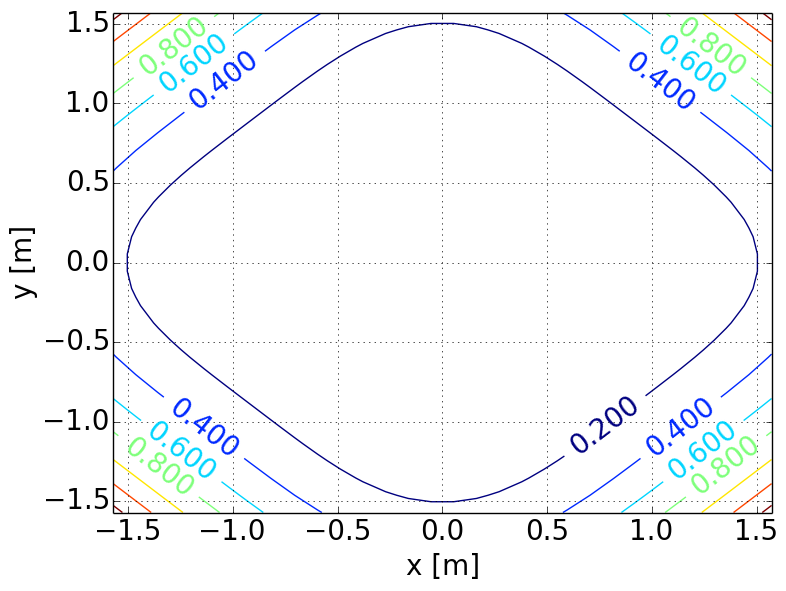
\includegraphics[width=\linewidth]{../4a_2_0,5_30.png}
        \caption{}
    \end{subfigure}
    \caption{Figurene viser $|x| < \frac{\pi}{2}$ og
    $|y| < \frac{\pi}{2}$ med $n = 30$.
    \color{blue} a) \color{black}
     viser konturlinjene
    til $\psi$.
    \color{blue} b) \color{black}
     viser konturlinjene til Taylor approksimasjon
    fra 3 e).
    \color{blue} c) \color{black}
     viser konturlinjene til forskjellen mellom a) og b).}
    \label{fig_4a_second}
\end{figure}

\pagebreak
\begin{figure}[H]
    \centering
    \begin{subfigure}{0.3\textwidth}
        \centering
        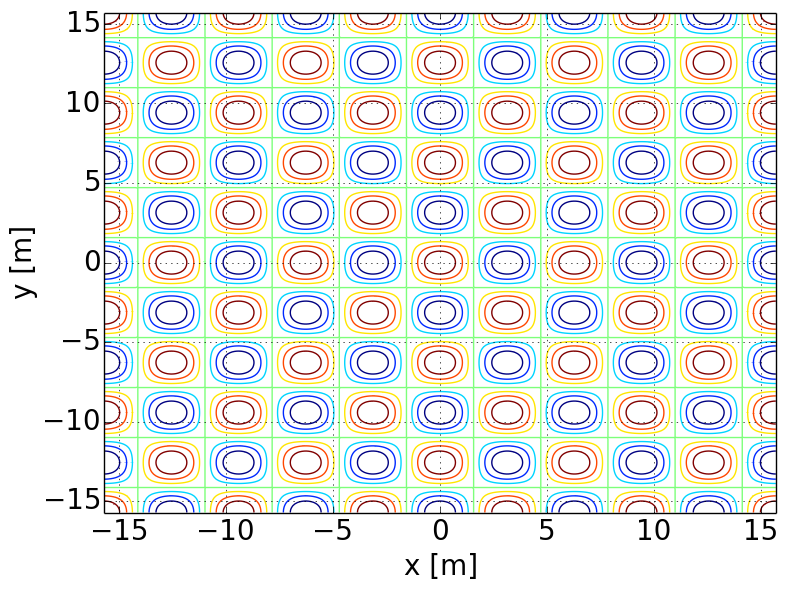
\includegraphics[width=\linewidth]{../4a_0_5_300.png}
        \caption{}
    \end{subfigure}%
    ~
    \begin{subfigure}{0.3\textwidth}
        \centering
        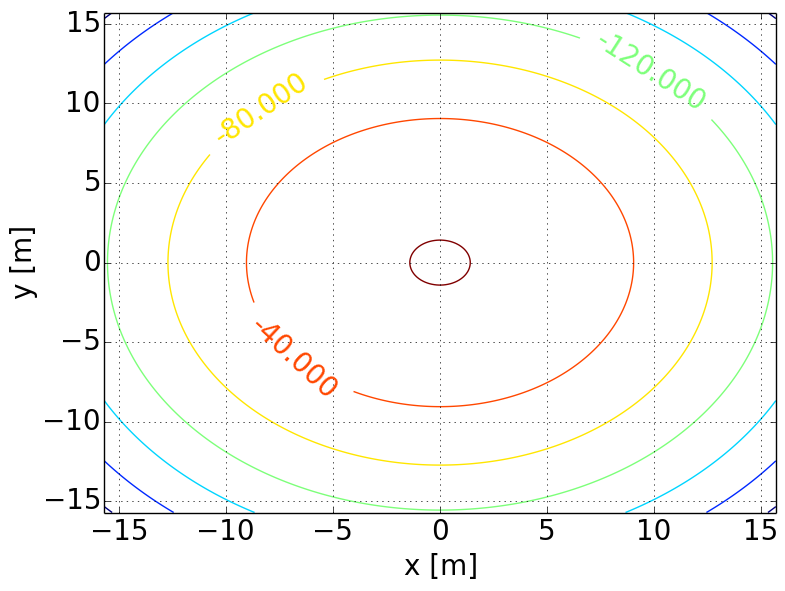
\includegraphics[width=\linewidth]{../4a_1_5_300.png}
        \caption{}
    \end{subfigure}
    ~
    \begin{subfigure}{0.3\textwidth}
        \centering
        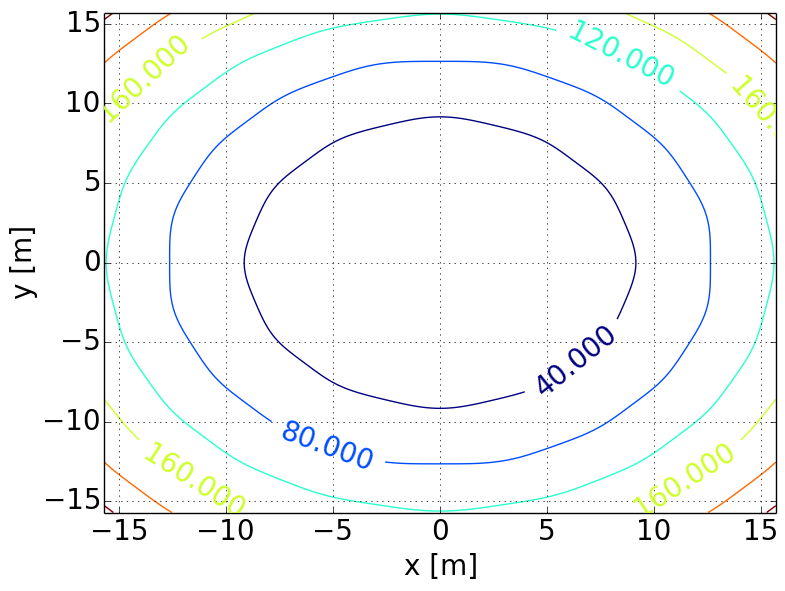
\includegraphics[width=\linewidth]{../4a_2_5_300.png}
        \caption{}
    \end{subfigure}
    \caption{Figurene viser $|x| < \frac{\pi}{2}$ og
    $|y| < \frac{\pi}{2}$ med $n = 30$. \color{blue} a) \color{black}
     viser konturlinjene til $\psi$. \color{blue} b)\color{black} viser
     konturlinjene til Taylor approksimasjon
    fra 3 e). \color{blue} c) \color{black} viser konturlinjene til forskjellen mellom a) og b).}
    \label{fig_4a_third}
\end{figure}

Vi ser at for den første svigningen i $\psi$ approksimasjonen fra
3 e) er ganske god. I figur \ref{fig_4a_first} og figur \ref{fig_4a_second}
vi kan se at det er kun en feil på sirka 0.2 når vi har
kommet til $\frac{\pi}{2}$ på aksene. Dette er å
forvente Taylor approksimasjonen skal være best nærmt
punktet tilnærmingen er laget. Selv om det ikke er blitt spurt om tar
jeg med et plott som viser verdiene til $\psi$ opp til $ 5 \pi $ på aksene
med n satt til 300. I figur \ref{fig_4a_third} kan vi se resultatet.
Jeg tar med dette, fordi det viser hvordan approksimasjonen kun er god rundt
toppen i origo, mens den er helt forferdelig på å tilnærme de andre toppene/bunnene.













\subsection*{4 b)}

\textbf{Skriv en funksjon (\sout{velfield.m eller} velfield.py) som
bergener hastigheter utfra likning (1) ved kallet $x,y,u,v = velfield(n)$.
\\
\\
Bruk denne i et skript, \sout{vec.m eller} vec.py, som tegner et vektorplott
av hastighetsfeltet. Legg vekt på å vlege et passende antall punkter for
lesbarheten av plottet.}

\begin{figure}[H]
    \centering
    \begin{subfigure}{0.5\textwidth}
        \centering
        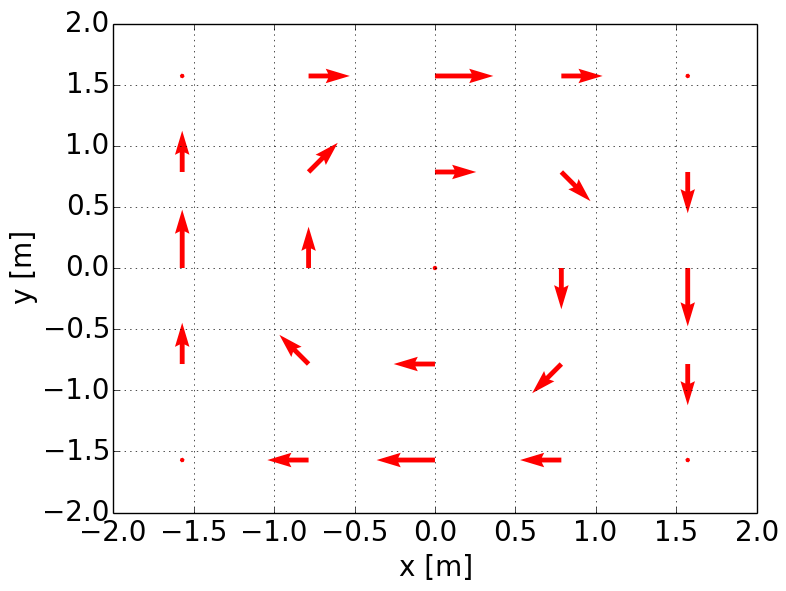
\includegraphics[width=\linewidth]{../4b5.png}
        \caption{}
    \end{subfigure}%
    ~
    \begin{subfigure}{0.5\textwidth}
        \centering
        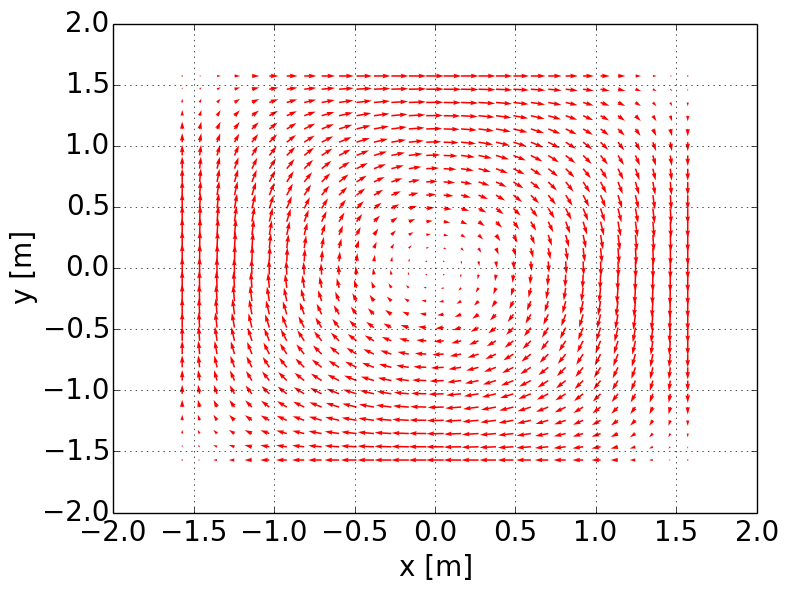
\includegraphics[width=\linewidth]{../4b30.png}
        \caption{}
    \end{subfigure}
    \caption{Figurene viser vektorplott av hastighetsfeltet
    ved hjelp av funksjonen definert i velfield.py. a) er vektorplottet med $n = 5$.
    b) er vektorplottet $n = 30$. }
    \label{fig_4b}
\end{figure}

Figur \ref{fig_4b} er laget ved scriptene beskrevet i oppgaveteksten.
Personlig liker jeg bedre figurer med mange piler (ser mer avansert ut), men
jeg legger ved to varianter slik at det er mer lesbart. 
